\chapter{Introducci�n}\label{capitulo1}

\section{Antecedentes}
Los antecedentes deben ser extensos pero, lo suficientemente cortos para ser entendidos por todos.

\section{Im�genes}
Las im�genes
\begin{figure}[!htb]
	\centering
	\begin{subfigure}[b]{0.4\textwidth}
		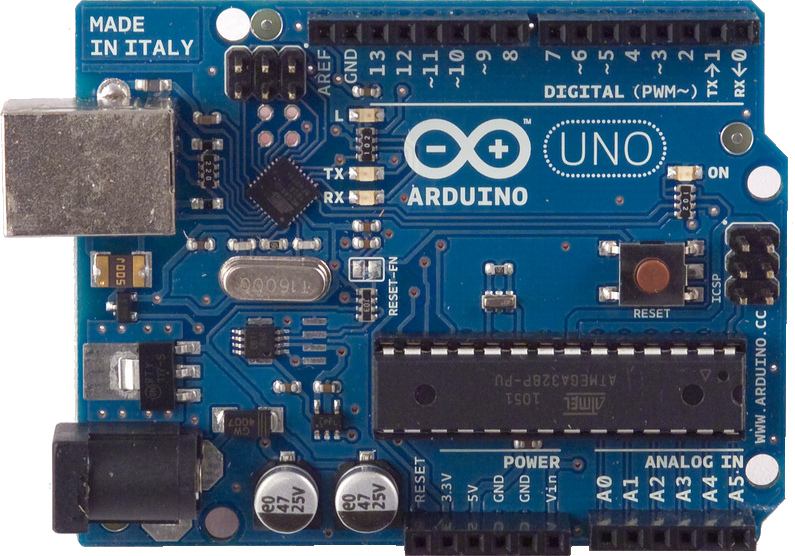
\includegraphics[width=\textwidth]{img/ArduinoUnofront.jpg}
		\caption{Primera imagen}
		\label{fig:gull}
	\end{subfigure}
	\begin{subfigure}[b]{0.4\textwidth}
		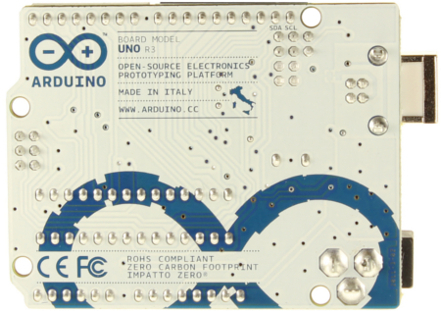
\includegraphics[width=\textwidth]{img/ArduinoUnoBack.jpg}
		\caption{Segunda imagen}
		\label{fig:tiger}
	\end{subfigure}
	\caption{Varias im�genes comparadas y con un propio \textbf{caption} para cada uno}
	\label{fig:animals}
\end{figure}